\section{Testing}
\label{sec:diffstream}

In this section we describe how the programmer writes specifications in DiffStream~\citeMain{oopsla20}.
Let's look back at the taxi example from before. The second stage of the program
computes the total distance traveled by each taxi by computing the
distance between the current and the previous location, and adding
that to a sum. For this computation to return correct results,
location events for each taxi should arrive in order in its input---a
requirement that must be checked if we want to test the first stage of
the program. We propose expressing this ordering requirement using a
\emph{dependence relation} $D$. The concept of dependence relations
was first introduced in research on concurrency theory, where it was
used to define Mazurkiewicz traces, i.e. partially ordered sequences
of events in distributed systems~\cite{mazurkiewicz1986trace},
and has previously been used to give semantics for stream processing programs~\cite{mamouras2019data}.

A dependence relation is a symmetric binary relation on events of a
stream with the following semantics.
If $x \dep y$, then the order of
$x$ and $y$ in a stream is significant and reordering them gives us
two streams that are not equivalent. This could be the case if the
consumer of an output stream produces different results depending on
the order of $x$ and $y$.  Thus, the dependence relation can be
thought of as encoding the pairwise ordering requirements of the
downstream consumer.

\begin{figure}[t]
  \centering \footnotesize{}
  \begin{subfigure}[b]{0.46\textwidth}
    \centering
    \begin{lstlisting}[basicstyle=\ttfamily\small]
  (ev1, ev2) ->
      ev1.taxiID == ev2.taxiID
    \end{lstlisting}
    \caption{Specification in DiffStream}
    \label{fig:simple-taxi-example-dependency-spec}
  \end{subfigure}%
  \qquad
  \begin{subfigure}[b]{0.46\textwidth}
    \centering
    \KeyDepGraph{tID}
    \caption{Dependence visualized as a graph}
    \label{fig:simple-taxi-example-dependency-vis}
  \end{subfigure}%
  \caption{Example specification in DiffStream for the taxi example. Taxi events with the same \inljava{taxiID} are dependent.}
  \label{fig:example-dependencies}
\end{figure}

It is often helpful to visualize dependence relations as unordered
graphs, where nodes are equivalence classes of the dependence
relation. For the taxi example, the dependence relation is visualized
in Figure~\ref{fig:simple-taxi-example-dependency-vis}, and it indicates that
events with the same taxi identifier are dependent. In DiffStream,
dependence relations can be specified using a Boolean function on a pair
of events. These functions should be pure and should only depend on
the fields of the two events. The DiffStream specification of the dependence relation from Figure~\ref{fig:simple-taxi-example-dependency-vis} is shown in Figure~\ref{fig:simple-taxi-example-dependency-spec}.

\begin{figure}[t]
  \centering \footnotesize{}
  \begin{subfigure}[b]{0.56\textwidth}
    \centering
    \begin{lstlisting}[basicstyle=\ttfamily\small,linewidth=7.3cm]
  (ev1, ev2) ->
      ev1.isEOD() ||
      ev2.isEOD() ||
      (ev1.isEOM() && ev2.isEOM()) ||
      (ev1.isTaxiEv() &&
       ev2.isTaxiEv() &&
       ev1.taxiID == ev2.taxiID)
    \end{lstlisting}
    \caption{Specification in DiffStream}
    \label{fig:extended-taxi-example-dependency-spec}
  \end{subfigure}%
  \qquad
  \begin{subfigure}[b]{0.36\textwidth}
    \centering
    \ExtendedKeyDepGraph{tID}
    \caption{Dependence visualized as a graph}
    \label{fig:extended-taxi-example-dependency-vis}
  \end{subfigure}
  \caption{Example specification in DiffStream for the extended taxi example. Taxi events with the same \inljava{taxiID} are dependent
      and all events are dependent with end-of-day (EOD) events.}
  \label{fig:extended-example-dependencies}
\end{figure}

Now let's consider an extension of the above example where the downstream consumer
computes the total distance traveled by each taxi \emph{per
  day}, and also computes the average daily distance by each taxi
every month. To make this possible, the output of the program under test
is now
extended with special EOD (\emph{end-of-day}) and EOM (\emph{end-of-month})
events. The ordering requirements on this output, while more subtle, can still be
precisely specified using a dependence relation.
For example, EOD events are dependent with taxi events since all events of a specific day have to occur before the EOD event of that day for the total daily distance to be correctly computed. On the other hand, EOM events do not have to be dependent with taxi events since daily distances are computed on EOD events. Therefore, an EOM event can occur anywhere between the last EOD event of the month and the first EOD event of the next month.
The DiffStream specification of the dependence relation and its visualization are both shown in Figure~\ref{fig:extended-example-dependencies}.

\begin{figure}[t]
  \centering \footnotesize{}
\begin{tabular}{c}
\begin{lstlisting}[basicstyle=\ttfamily\small,linewidth=9cm]
  (ev1, ev2) -> distance(ev1.loc, ev2.loc) < 1
\end{lstlisting}
\end{tabular}
  \caption{Example specification in DiffStream where  events are dependent if their locations are close.}
  \label{fig:proximity-example-dependencies}
\end{figure}

Several frequently occurring dependence relations can be specified
using a combination of the predicates seen in the above examples. This
includes predicates that check if an event is of a specific type
(e.g. \inljava{isEOD()}, \inljava{isTaxiEv()}), and predicates that
check a field (possibly denoting a key or identifier) of the two
events for equality (e.g. \inljava{ev1.taxiID ==
  ev2.taxiID}). However, it is conceivable that the dependence of two
events is determined based on a complex predicate on their fields.

\begin{figure}[t]
  \centering \footnotesize{}
\begin{tabular}{c}
\begin{lstlisting}[basicstyle=\ttfamily\small,linewidth=10cm]
  (ev1, ev2) -> (ev1.isPunctuation() &&
                 ev2.timestamp < ev1.timestamp) ||
                (ev2.isPunctuation() &&
                 ev1.timestamp < ev2.timestamp)
\end{lstlisting}
\end{tabular}
  \caption{Example specification in DiffStream where punctuation events, used to enforce progress, depend on other events only if the punctuation timestamp is larger.}
  \label{fig:punctuation-example-dependencies}
\end{figure}

Another interesting dependence relation occurs in cases where output streams contain punctuation events.
Punctuations are periodic events that contain a timestamp and indicate
that all events up to that timestamp, i.e. all events \inljava{ev} such that \inljava{ev.timestamp < punc.timestamp}, have \emph{most likely} already occurred.
Punctuation events allow programs to make progress, completing any
computation that was waiting for events with earlier
timestamps. However, since events could be arbitrarily delayed, some
of them could arrive after the punctuation.
Consider as an example a taxi that briefly
disconnects from the network and sends the events produced while disconnected
after it reconnects with the network. These events are usually
processed with a custom out-of-order handler, or are completely
dropped. Therefore, punctuation events are dependent with events
that have an earlier timestamp, since reordering them alters the result of the computation, while they are independent of events with later timestamps. This can be specified in DiffStream as
shown in Figure~\ref{fig:punctuation-example-dependencies}.

\begin{algorithm}[t]
  \renewcommand{\thealgorithm}{DiffStream}
  \caption{Checking equivalence of two streams}
  \label{alg:equivalence}
  \begin{algorithmic}[1]
    \Require Equality relation $\equiv$, dependence relation $\dep$
    \Require Connected stream $s$ with $\pi_1(s)=s_1$ and $\pi_2(s)=s_2$
    \renewcommand{\algorithmicrequire}{\textbf{Require:}}
    \Require Relations $\equiv$ and $\dep$ are compatible
    \Function{StreamsEquivalent}{$s$}
    \label{line:StreamsEquivalentBegin}
    \State $u_1, u_2 \gets$ empty logically ordered sets
    \State {\color{gray}Ghost state: $p_1, p_2 \gets$ empty logically ordered sets}
    \State {\color{gray}Ghost state: $f \gets$ empty function $p_1\to p_2$}
    \For{$(x, i)$ in $s$}\label{line:ProcessElementBegin}
      \State $j \gets 3-i$
      \If{$x$ is minimal in $u_i$ and $\exists y\in \min u_j: x \equiv y$}
      \label{line:MatchBegin}
        \State $u_j \gets u_j \setminus \{y\}$
        \State {\color{gray}$p_i \gets p_i \cup \{x\}$};
        {\color{gray}$p_j \gets p_j \cup \{y\}$}\label{line:GhostBegin}
        \State {\color{gray}$f \gets f[x\mapsto y]$ \textbf{if} $i=1$
          \textbf{else} $f[y\mapsto x]$}\label{line:MatchEnd}
      \ElsIf{$\exists y \in u_j: x \dep y$}\label{line:NotEquivalentBegin}
        \State \textbf{return false}\label{line:NotEquivalentEnd}
      \Else\label{line:UnmatchedBegin}
        \State $u_i \gets u_i \cup \{x\}$\label{line:UnmatchedEnd}
      \EndIf\label{line:ProcessElementEnd}
    \EndFor
    \State \textbf{return} ($u_1=\emptyset$ and $u_2=\emptyset$)
    \label{line:FiniteEquivalent}
    \EndFunction\label{line:StreamsEquivalentEnd}
  \end{algorithmic}
\end{algorithm}

\begin{figure}[tb]
    \centering \small
\begin{tabular}{c}
\begin{lstlisting}[linewidth=9.5cm]
public void testKeyBy() throws Exception {
    StreamExecutionEnvironment env = ...;

    DataStream input = generateInput(env);

    StreamEquivalenceMatcher matcher =
        StreamEquivalenceMatcher.createMatcher(
            sequentialImpl(input), parallelImpl(input),
            (ev1, ev2) -> ev1.taxiID == ev2.taxiID);

    env.execute();
    matcher.assertStreamsAreEquivalent();
}
\end{lstlisting}
\end{tabular}
    \caption{An example test in DiffStream.}
    \label{fig:keybytest}
\end{figure}{}

\begin{figure}[tb]
    \centering \small

    \setlength\tabcolsep{1em}
    \begin{tabular}{c|ccc}
          & \multicolumn{3}{c}{\underline{Application-Specific Requirements}} \\
         Code pattern & Determinism & \makecell{Determinism under \\ input assumptions} & \makecell{None \\ (nondeterminism acceptable)} \\
         \hline
         \texttt{SingleItem} & \cmark{} & \cmark{} & n/a \\
         \texttt{IndexValuePair} & \cmark{} & \cmark{} & n/a \\
         \texttt{MaxRow} & \cmark{} & \cmark{} & \xmark{} \\
         \texttt{FirstN} & \cmark{} & \cmark{} & \xmark{} \\
         \texttt{StrConcat} & \cmark{} & n/a & \cmark{} \\
    \end{tabular}

    \caption{Results of the MapReduce case study. A \cmark{} indicates successfully identifying the bug in the first column, and successfully avoiding a false positive in the second and third columns, for each of the 5 reducers implemented.}
    \label{fig:mapreduce-case-study-summary}
\end{figure}

\begin{figure}[t!]
    \centering
    \begin{subfigure}[t]{0.33\textwidth}
        \centering
        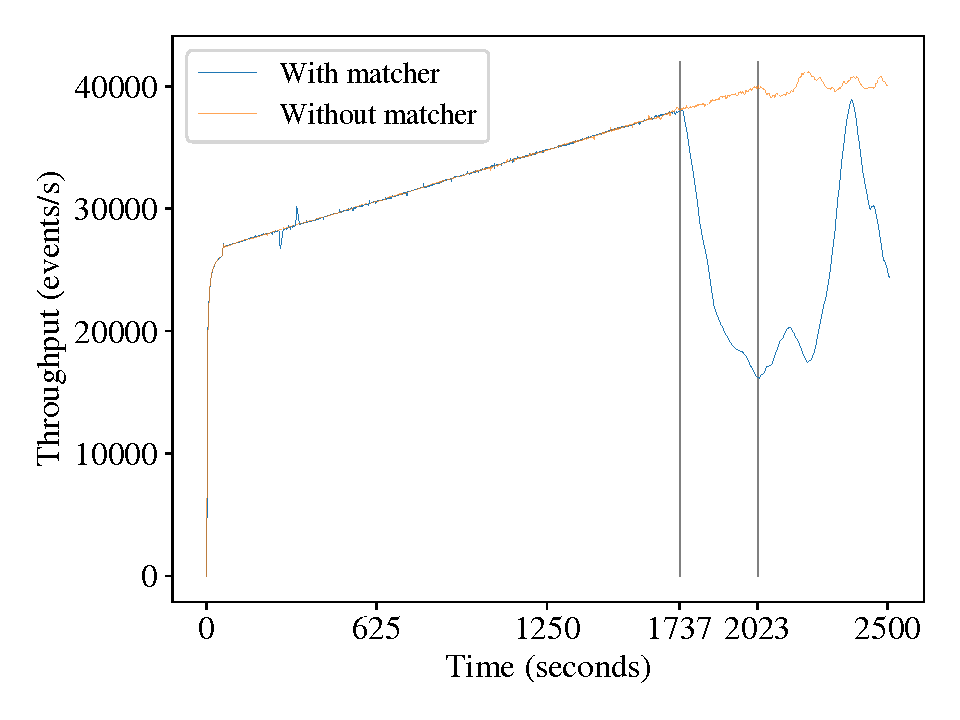
\includegraphics[width=1.0\textwidth]{figures/diffstream/throughput-accelerated.pdf}
        \caption{}\label{fig:throughput}
    \end{subfigure}%
    \begin{subfigure}[t]{0.33\textwidth}
        \centering
        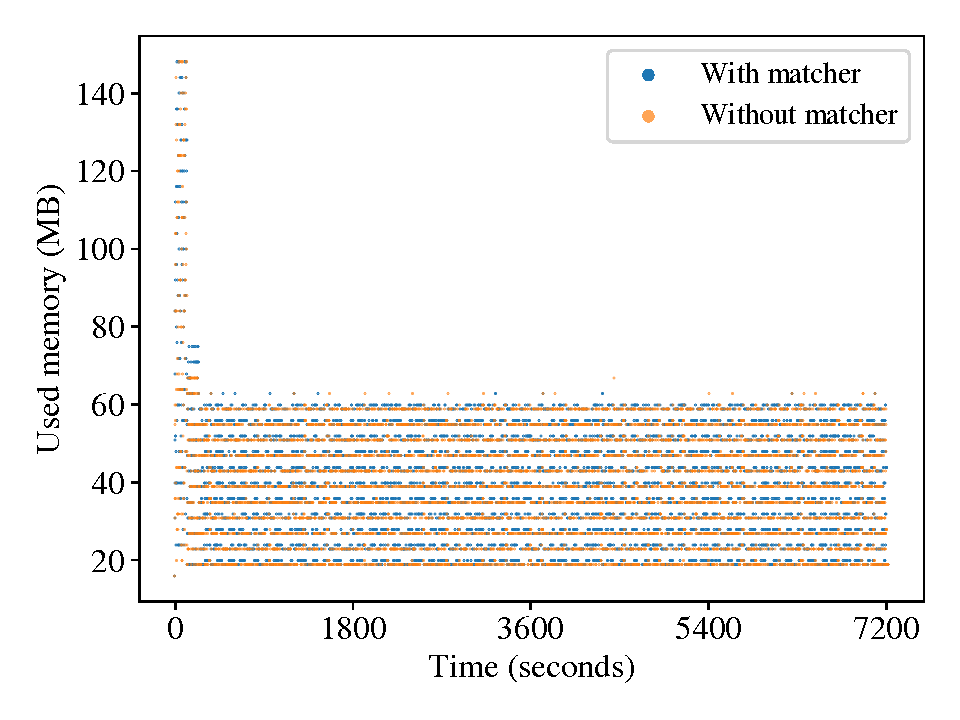
\includegraphics[width=1.0\textwidth]{figures/diffstream/used_memory_in_time.pdf}
        \caption{}\label{fig:memory-in-time}
    \end{subfigure}%
    \begin{subfigure}[t]{0.33\textwidth}
        \centering
        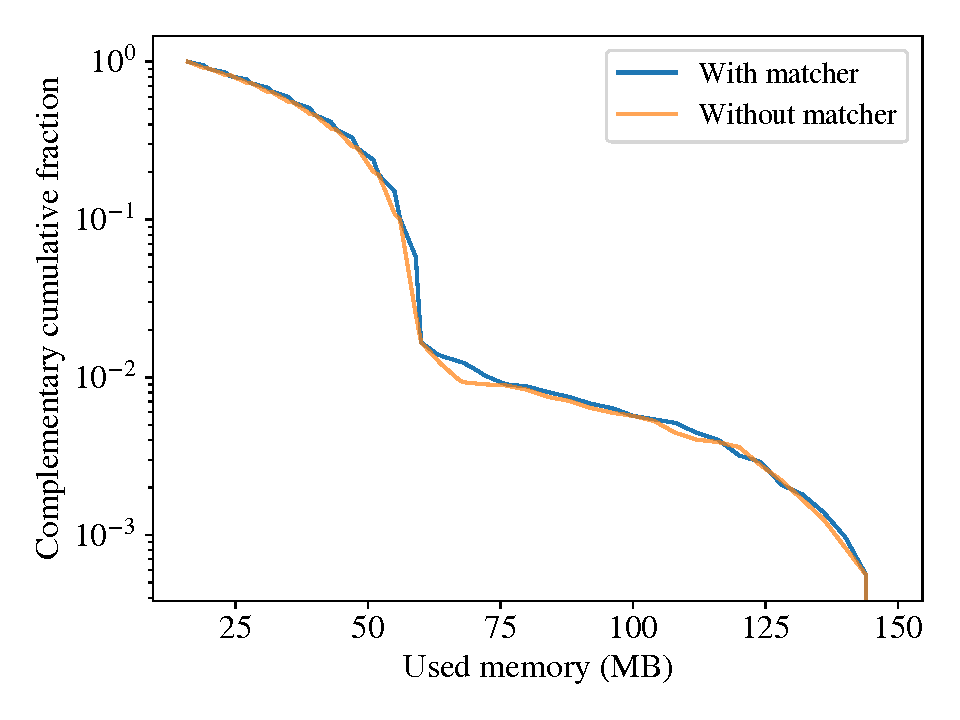
\includegraphics[width=1.0\textwidth]{figures/diffstream/memory_ccdf.pdf}
        \caption{}\label{fig:memory-ccdf}
    \end{subfigure}%
    \\
    \begin{subfigure}[t]{0.33\textwidth}
        \centering
        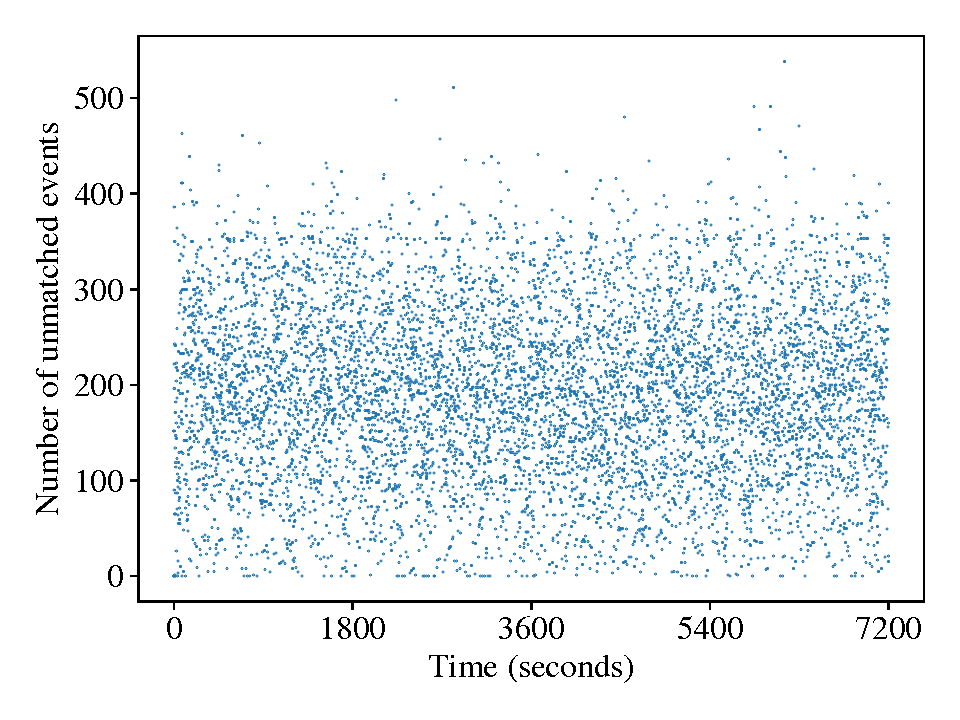
\includegraphics[width=1.0\textwidth]{figures/diffstream/unmatched_in_time.pdf}
        \caption{}\label{fig:unmatched-in-time}
    \end{subfigure}%
    \begin{subfigure}[t]{0.33\textwidth}
        \centering
        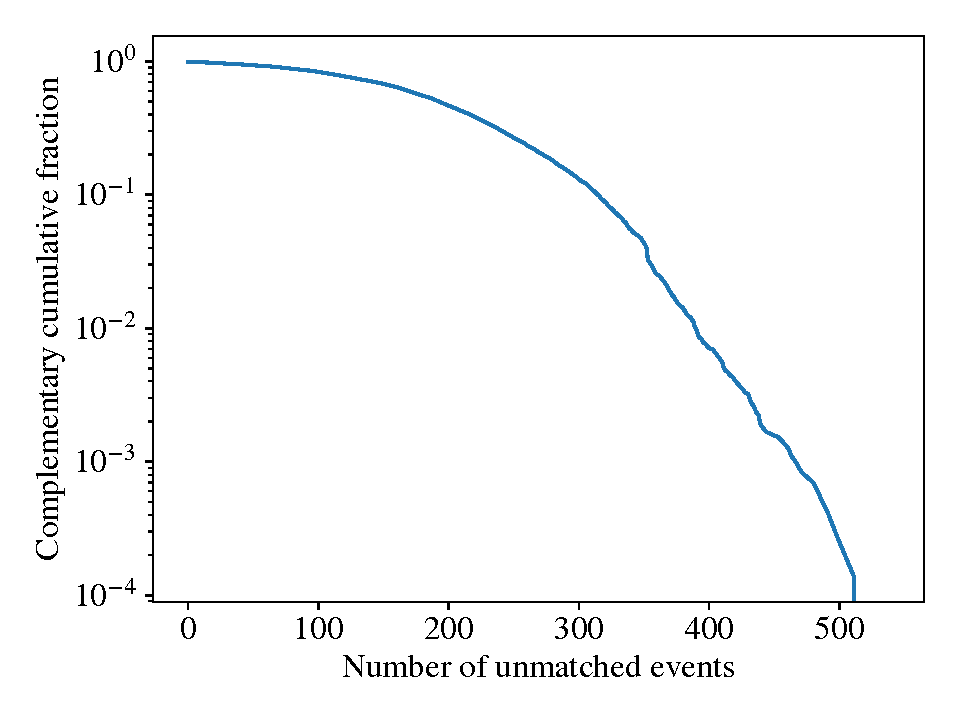
\includegraphics[width=1.0\textwidth]{figures/diffstream/unmatched_ccdf.pdf}
        \caption{}\label{fig:unmatched-ccdf}
    \end{subfigure}%
    \begin{subfigure}[t]{0.33\textwidth}
        \centering
        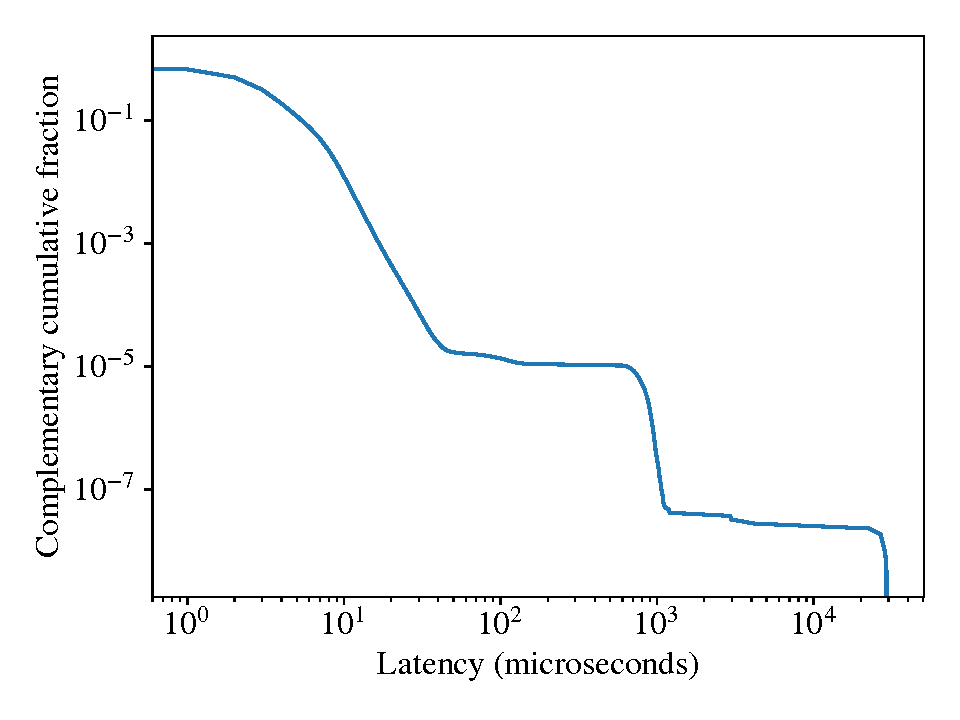
\includegraphics[width=1.0\textwidth]{figures/diffstream/latencies.pdf}
        \caption{}\label{fig:latencies}
    \end{subfigure}
    \caption{Results of the fourth case study: performance measurements of monitoring an application with DiffStream on the Yahoo streaming benchmark over a span of 2 hours, compared to the same application without the DiffStream matcher.}
\label{fig:online-perf-results}
\end{figure}
